\chapter{Implementation}
\label{Chapter4}
% Main chapter title
\lhead{Chapter 2. \emph{Implementation}}

This Chapter presents the implementation overview of our approach. Section \ref{selectingCandidates} presents an outline about selecting suitable Selenium test-suites for our research. Section \ref{implementationsetup} discusses the implementation and infrastructural setup necessary to evaluate the robustness of Selenium test-suites. 

% Section \ref{infra} does infra, Section \ref{stateModelExtraction} extracts state models using webmate. \ref{selectingCandidates} selects candidates, Section bleh}

% All subsections start from here onwards:
\section{Selenium Test-suites}
\label{selectingCandidates}
In order to evaluate the robustness of Selenium tests, our objective was to empirically investigate different open-source web applications that have publicly available Selenium test-suites. The idea was that open-source Selenium tests generally have multiple contributors, which will provide a richer and unbiased data set as compared to tests written by a single individual. Adhering to this idea, the first step is to select suitable test candidates that satisfy a certain set of requirements for this research. 

According to the approach presented in Section \ref{robustnessOfSeleniumTests}, the first requirement for the test candidates is to have a sufficiently long development history, preferably with major versions and minor revisions. The reason for selecting open-source applications is that the older versions/releases of their applications are usually available for public usage. Availability of different releases is essential for this thesis since we are evaluating the robustness over the version history of web applications. In case there is no clear distinction made between major and minor releases for certain applications, we plan to resort to other options for identifying different releases, such as checking out tags or commits from version control repositories. 

The second requirement for candidates fulfilling above requirements is to have publicly available Selenium test-suites with a minimum of ten Selenium tests. A test number below that would not be sufficient for this analysis. As mentioned in Chapter \ref{Chapter2}, this thesis considers Selenium \texttt{webdriver} based tests. These tests can be run using the \texttt{RemoteWebdriver} implementation and are to be integrated with the tool \texttt{webmate} as we will see in Section \ref{stateModelExtraction}. Additionally, preference is given to the test-suites which are being developed in parallel to their respective web applications, to evaluate the approach presented in Section \ref{locatorMaintenance}. Moreover, our implementation considers tests available in all supported languages, such as Java, Python, etc. 

To identify whether given test-suite is suitable for our analysis, we locally deploy the AUT, execute the Selenium tests on it and record the test outcome. Some tests are designed specifically for an organization's internal testing servers or may require certain configurations not available for public use. In other words, not all tests from a test-suite are expected to work on locally deployed instances. In such cases, we record the number of tests that are suitable for running locally and consider them for our analysis. 


% \subsubsection{Candidate Selection}
\section{Implementation setup}
\label{implementationsetup}
As we have seen in Chapter \ref{Chapter1}, Figure \ref{fig:thesisoverview2} depicts the setup required for the robustness analysis of selected test candidates. The following sections provide a brief overview of different steps of this implementation setup.  
\begin{figure}[h]
% [htbp]
	\centering	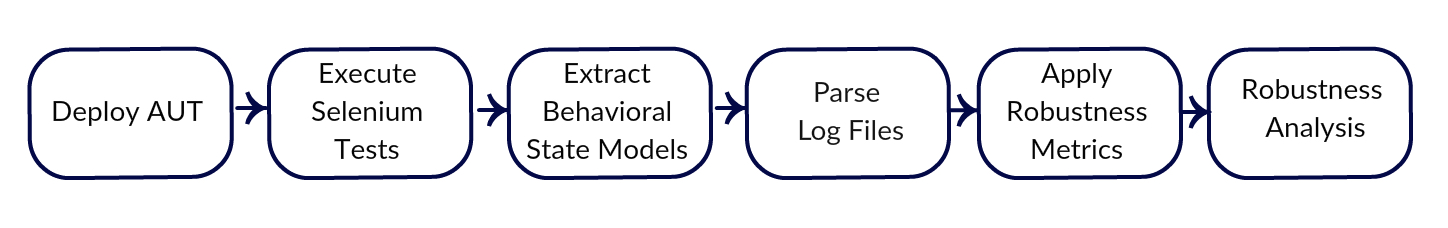
\includegraphics[width=\textwidth]{./Figures/thesisoverviewsmall.jpg}
%     [width=5cm, height=3cm]
% 		\rule{35em}{0.5pt}
	\caption{Setup required for the robustness analysis}
	\label{fig:thesisoverview2}
\end{figure} 

\subsection{Automated Application Deployment}
\label{sec:autoDeployment}



% \section{Web Application Deployment}

To measure the robustness of Selenium tests across different versions of AUT, the first step of the implementation setup is to make these versions accessible for the testing setup as shown in Figure \ref{fig:thesisoverview2}. It is possible to accomplish this by installing and deploying these versions locally (without relying on external application server provider). Generally, most of the open-source application vendors make older versions of their applications available for public usage. The most common ways to release such web applications are by releasing packaged versions ready to deploy, such as \texttt{war} (Web application ARchive) files in case of Java applications, by checking out the code from version control repositories such as git, subversion, mercurial etc.

\begin{figure}[h]
\makeatletter 
% \renewcommand{\thefigure}{\@arabic\c@figure}
\makeatother
% \setcounter{figure}{0}
    \centering
  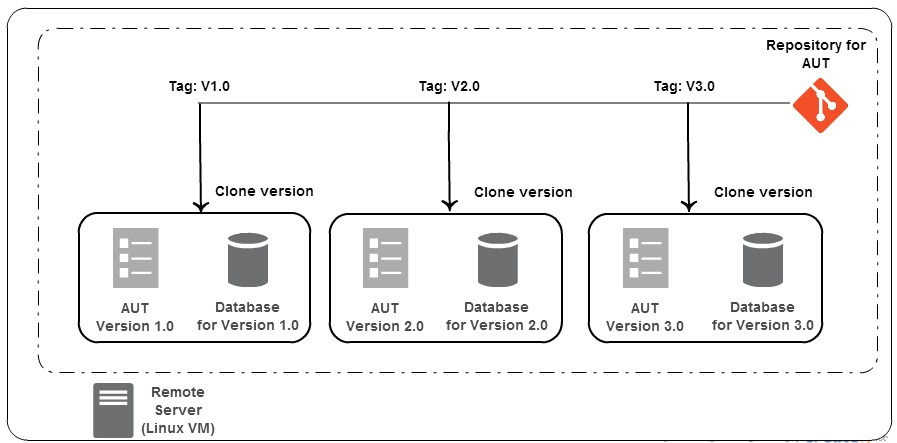
\includegraphics[width=5.4in,height=2.6in]{./Figures/Deployment_Process_2.jpg}
  \captionsetup{justification=raggedright,
singlelinecheck=false
}
  \caption{Automatic deployment workflow to deploy multiple instances (versions) of AUT in parallel}
  \label{fig:deployment} 
\end{figure}

Depending upon the type of the web application, the frameworks and programming languages used to create these application, different set of application servers can be used for deploying the AUT. Java based packaged applications such as \texttt{war} archives can be deployed in Java containers such as Tomcat\footnote{\url{http://tomcat.apache.org/}}. Similarly, PHP based applications can be hosted inside Apache httpd\footnote{\url{https://httpd.apache.org/}} servers. 

The AUT can be installed as per the installation instructions provided by the application vendors. The installation setup includes steps such as downloading the application source code or packaged binaries, creating databases and other configurations etc. Certain Selenium tests require the AUT to have some pre-configured features enabled, such as an \textit{administrative} user account setup which can also be accomplished in the installation phase. 

In order to spare the manual effort of installing multiple versions of AUT and to be able to reproduce our results, we have automated the deployment work-flow through automated deployment scripts. In order to speed up the testing process, we plan to deploy multiple versions of the AUT in parallel and sand-boxed inside a secure Linux based virtual machine for security reasons. Figure \ref{fig:deployment} depicts the overview of remote automatic deployment process; three versions of the AUT are running simultaneously against their individual database instances.

% \subsection{Automatic application deployment}
\subsection{Behavioral State Models}
\label{stateModelExtraction}
Subsequently, the next steps (see Figure \ref{fig:thesisoverview2}) are to execute the Selenium tests on the AUT and extract the behavioral state models. In order to measure the \textit{robustness grade} of a test across two different versions, it is essential to verify whether the test covers same functional states across both versions. For this purpose, the behavioral state models are compared to check if same states of the AUT are reached by the test. 

\begin{figure}[h]
\makeatletter 
% \renewcommand{\thefigure}{\@arabic\c@figure}
\makeatother
    \centering
  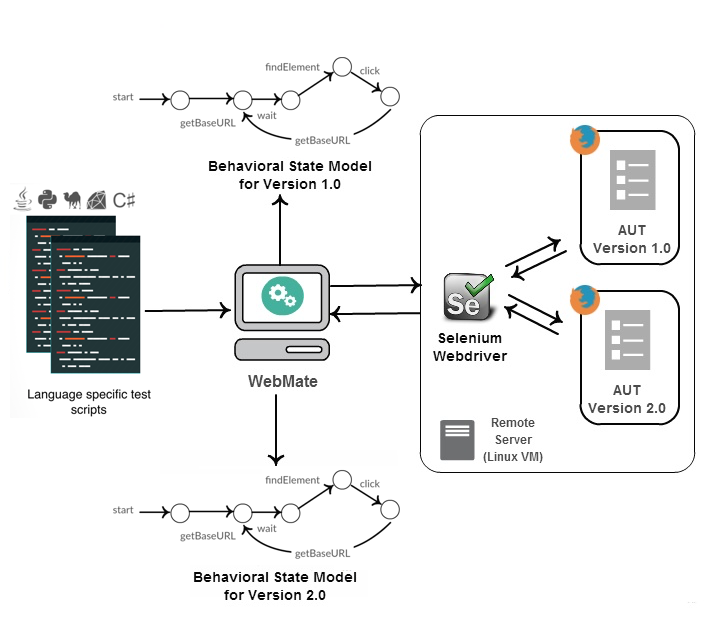
\includegraphics[width=5.5in,height=4.5in]{./Figures/WebMate_state_extraction.png}
% \begin{flushleft}

\caption{Extraction of behavioral state models using \texttt{webmate}}
% \end{flushleft}
 \label{fig:webmateExtraction} 
\end{figure}

As mentioned in Section \ref{sec:WebMate}, \texttt{webmate} can leverage existing Selenium tests to extract a behavioral state model (usage-model) of the AUT. Figure \ref{fig:webmateExtraction} depicts the process of extracting behavioral state models by integrating the test scripts with \texttt{webmate}. Two different versions of an application are deployed in parallel as per the process as described in Section \ref{sec:autoDeployment}. For security reasons, Selenium tests are integrated with \texttt{webmate} inside a virtual machine that hosts a Selenium hub. With this setup, \texttt{webmate} supports multiple testing instances by using the \texttt{RemoteWebDriver} capabilities for communicating with the Selenium test scripts. The Selenium test scripts and the base URL of the application are given as input to \texttt{webmate} as it can simultaneously execute the test scripts on different versions of the AUT to generate the behavioral state models. For each state of the behavioral state model, \texttt{webmate} is able to record its visual (GUI) state, in the form of a screen-shot of the AUT. Essentially, the states of the state model represent the DOM state of the AUT, and the transitions represent the \textit{actions} executed by the test on the AUT.

Every state model is uniquely identified by the browser \textit{sessionId} associated with each test session. As an example, let us revisit the \texttt{loginTest} we have seen in Listing \ref{code1}. When the \texttt{loginTest} is executed with \texttt{webmate}, its state model resembles the structure in Listing \ref{statemodellisting}. Each action executed by the test (e.g. a \texttt{findElement} request) can be identified by the \textit{sessionId} of the test. However, at this point it is important to mention that the behavioral state model can only capture \texttt{wait} commands which have a \textit{fixed} duration, such as \texttt{implicitlyWait} conditions. Commands with uncertain duration, such as \texttt{wait.until} conditions cannot be captured within the model and therefore it is not possible to evaluate them in this thesis. 

\begin{center}
\begin{scriptsize}
\centering
\lstset{
  basicstyle=\ttfamily,
  columns=fullflexible,
  keepspaces=true,
%   frame=none,
}
% \verb|basicstyle=\ttfamily, columns=fullflexible, keepspaces=true|
  
\begin{lstlisting}[caption=Extracted behavioral state model for \texttt{loginTest},label=statemodellisting]
 actions : { 
[session-Id, get {url="http://application-under-test.com"}]
},
 actions : { 
[session-Id, findElement {using="id", value="uname"}]
},
 actions : { 
[session-Id, sendKeysToElement {id="1", value=["user"]}],
[session-Id, findElement {using="id", value="pwd"}]
},
 actions : { 
[session-Id, sendKeysToElement {id="2", value=["passwd"]}],
[session-Id, findElement {using="link text", value="Login"}]
},
 actions : { 
[session-Id, clickElement {id="3"}]
}
\end{lstlisting}
\end{scriptsize} 
\end{center}

% level differences between the reference version and the subsequent versions (e.g. minor revisions) of the AUT. 
% \subsection{Comparing Behavioral State Models}
\subsection{Tool Implementation}
\label{toolimplementation}
This section presents an overview of the implementation process. In order to evaluate the approaches presented in Chapter \ref{Chapter3}, a tool has been implemented in Python language. 

\textbf{To answer RQ1}, it is necessary to assess whether a test covers the same states for different versions of the AUT. As mentioned in Section \ref{robustnessOfSeleniumTests}, the approach is to measure the  \textit{robustness grade} ($R_{T_{V_{0}V_{1}}}$) of test \textit{T} for a newer version \textit{$V_{1}$} compared against the reference version \textit{$V_{0}$}. Initially, test \textit{T} is executed on reference version \textit{$V_{0}$} and the behavioral state model \textit{$M_{0}$} is extracted and stored as shown in Listing \ref{stateModelExtraction}. Thereafter, test \textit{T} is executed on newer version \textit{$V_{1}$} in similar manner and the state model \textit{$M_{1}$} is recorded as well.

In the next step, for determining the \textit{robustness grade} we perform an equivalence check of the states of the behavioral models  \textit{$M_{0}$} and \textit{$M_{1}$} for reference and test versions \textit{$V_{0}$} and \textit{$V_{1}$} respectively.  
In order to perform the equivalence check, both the DOM level as well as GUI level states are compared. The presented tool parses the extracted state models and compares the states and transitions across them. For comparing the GUI states, \textit{ImageMagick Convert}\footnote{http://www.imagemagick.org/script/convert.php} -- a command-line tool, has been used in combination of the presented tool. The GUI states are compared by the juxtaposition of two screen-shots. 

If both state models are equivalent then the test covers the same functionality across  \textit{$V_{0}$} and \textit{$V_{1}$}, and it is therefore robust. If the states of the behavioral models do not match, the test is marked as non-robust. In this manner, \textit{robustness grade} for each test in the test-suite (\textit{$T_1$,$T_2$..,$T_n$ $\in$ TS}) is calculated. For non-robust tests, the test execution results such as \textit{stack-traces} are examined to identify the reasons behind non-robust tests, such as \texttt{webdriver} exceptions \cite{SeleniumExceptions} and errors reported by the test. 

\textbf{To answer RQ2}, the approach is to examine the influence of the proposed \textit{robustness metrics } (see Section \ref{robfactors}) on the robustness \textit{ground truth} established in Section \ref{robustnessOfSeleniumTests}. The robustness metrics and the ground truth are represented as a feature matrix extended with a solution vector, as detailed in Section \ref{sec:Statistical}. 

For developing the feature matrix, a test-suite with \textit{n} tests \textit{$T_1$,$T_2$..,$T_n$ $\in$ TS} is executed on reference version \textit{$V_{0}$} and the behavioral state model is captured, similar to the model represented in Listing \ref{statemodellisting}. This behavioral model is further analyzed to extract the robustness metrics. 

The solution vector is calculated for each test from the \textit{ground truth} according to Definition \ref{robustness-ground-truth}. This feature matrix is used for estimating the Spearman's correlation coefficient between the features and the solution vector. To identify the most influential features, the \textit{lasso} regression method is applied, as described in Section \ref{sec:Statistical}. 

\textbf{To answer RQ3}, our approach is to measure the \textit{maintenance metrics} in terms of the number of GUI element locators as well as \texttt{wait} commands repaired between two successive revisions of the AUT, as described in Section \ref{locatorMaintenance}.

In many software development environments, the Selenium tests-suite is maintained in parallel to the development of the web applications. In other words, when a test-suite needs to be repaired, it is often repaired following the changes in the AUT. In this manner, different versions (\textit{$V_1,...,V_n$}) of the application can have corresponding versions of Selenium test-suites (\textit{$TS_1,...,TS_n$}). To measure the proposed maintenance metrics, each version $TS_1,...,TS_n$ of the test-suite is executed against corresponding version $V_1,...,V_n$ of the AUT and the behavioral state models \textit{$M_1,...,M_n$} at the test-suite level of the execution are recorded. Afterwards, the behavioral state models for these versions are compared in a pair-wise form, i.e. .  

Note that it is also possible that a test-suite is not repaired after a release because all the tests were robust. In such cases, we consider that a given version $V_1$ does not have a corresponding test-suite version $TS_1$. This indicates that there was no change in the maintenance metrics for this version of the test-suite. 
